%%% Local Variables:
%%% mode: latex
%%% TeX-master: t
%%% End:
\documentclass[]{article}
\usepackage[utf8]{inputenc}
\usepackage[upright]{fourier}
\usepackage{tikz}
\usetikzlibrary{matrix,arrows,decorations.pathmorphing}
\begin{document}


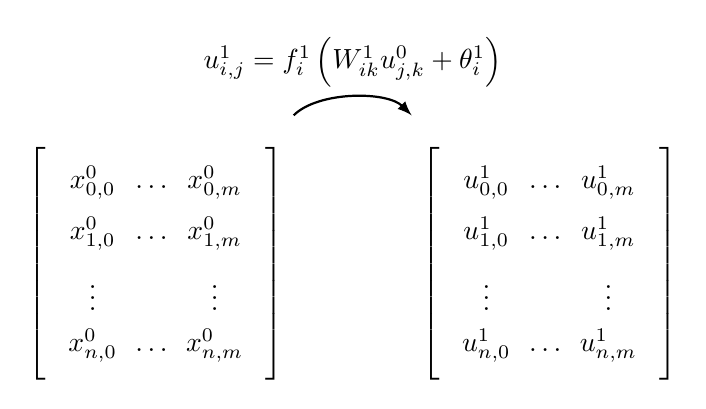
\begin{tikzpicture}[>=latex]
% les matrices
\matrix (A) [matrix of math nodes,%
             left delimiter  = {[},%
             right delimiter = {]}] at (0, 0)
{%
  x^0_{0,0} & \ldots & x^0_{0,m}  \\
  x^0_{1,0} & \ldots & x^0_{1,m}  \\
   \vdots &        & \vdots   \\
  x^0_{n,0} & \ldots & x^0_{n,m}  \\
};

\matrix (B) [matrix of math nodes,%
             left delimiter  = {[},%
             right delimiter = {]}] at (5, 0)
{%
  u^1_{0,0} & \ldots & u^1_{0,m}  \\
  u^1_{1,0} & \ldots & u^1_{1,m}  \\
   \vdots &        & \vdots   \\
  u^1_{n,0} & \ldots & u^1_{n,m}  \\
};


    \draw [->,thick, out=45,in=135,looseness=0.75]%
    ([xshift=0.4cm, yshift=0.4cm]A.north east) to%
    node[above]{$u^1_{i,j} = f^1_i\left( W^1_{ik} u^0_{j,k} + \theta^1_i \right)$}%
    ([xshift=-0.4cm, yshift=0.4cm]B.north west);

\end{tikzpicture}
\end{document}